\documentclass{article}
\usepackage{amsmath}
\usepackage{amssymb}
\usepackage{enumitem}
\usepackage{algorithm}
\usepackage{listings}
\usepackage{color,xcolor}
\usepackage[T1]{fontenc}
\usepackage{etoolbox}
\usepackage{multicol}
\usepackage{geometry}
\usepackage[colorlinks=true,linkcolor=blue,urlcolor=red,bookmarksopen=true]{hyperref}
\usepackage{tikz, pgfplots, tkz-euclide,calc}
    \usetikzlibrary{patterns,snakes,shapes.arrows,3d,patterns.meta,angles,quotes}
    \geometry{
        total = {160mm, 237mm},
        left = 25mm,
        right = 35mm,
        top = 30mm,
        bottom = 30mm,
      }

\usepackage{tcolorbox}
     \tcbuselibrary{listings,skins}

\newcommand{\enter}{\raisebox{-1.8pt}{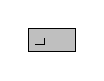
\begin{tikzpicture}[scale=0.3]
    \draw[thin,fill=lightgray] (0,0) rectangle (2,1);
    \draw (0.3,0.3) -- (0.7,0.3)--(0.7,0.6);     
\end{tikzpicture}}}

\definecolor{HIMAmuda}{HTML}{01D1FD}
\definecolor{HIMAtua}{HTML}{02016A}
\definecolor{HIMAabu}{HTML}{CBCBCC}
\definecolor{pgray}{rgb}{0.5,0.5,0.5}
\definecolor{pblue}{rgb}{0.13,0.13,1}
\definecolor{pgreen}{rgb}{0,0.5,0}
\definecolor{pred}{rgb}{0.9,0,0}
\definecolor{pgrey}{rgb}{0.46,0.45,0.48}
\definecolor{pcyan}{HTML}{D4EFFC}
\definecolor{lblue}{HTML}{00AEEF}
\definecolor{input}{HTML}{AAE1FA}
\definecolor{bg}{rgb}{0.95, 0.95, 0.92}
\definecolor{vscode}{HTML}{282A36}
\definecolor{PastelGreen}{HTML}{77DD77}

\newcommand{\inputscan}[1]{\raisebox{0pt}[1pt]{\colorbox{darkgray}{#1}}}

\usepackage{listings}

\lstdefinestyle{Liang}{
language=Java,
showspaces=false,
showtabs=false,
breaklines=true,
showstringspaces=false,
breakatwhitespace=true,
commentstyle=\color{pgray},
keywordstyle=\color{pblue},
stringstyle=\color{pgreen},
basicstyle=\small\ttfamily,
frame=single,
backgroundcolor=\color{pcyan},
escapeinside={(*}{*)},}

\lstdefinestyle{output}{
    language=Java,
    backgroundcolor=\color{vscode},
    basicstyle=\small\ttfamily\color{white},
    frame=none,
    escapeinside={(*}{*)},
    showspaces=false,
    showtabs=false,
    breaklines=true,
    showstringspaces=false,
    breakatwhitespace=true,
    keywordstyle=\color{white},
    }

\lstdefinestyle{standard}{
    language=Java,
    showspaces=false,
    showtabs=false,
    breaklines=true,
    showstringspaces=false,
    breakatwhitespace=true,
    commentstyle=\color{pgray},
    keywordstyle=\color{pblue},
    stringstyle=\color{pgreen},
    basicstyle=\small\ttfamily,
    frame=single,
    backgroundcolor=\color{bg},
    escapeinside={(*}{*)},}
\lstset{style=Liang}

\newtcblisting{RunCode}[1][enhanced,drop shadow]{
    arc=0pt, outer arc=0pt,
    boxsep=1pt,
    boxrule=2pt,
    auto outer arc,
    colback=vscode,
    colframe=bg,
    listing only, 
    listing style=output,
    title=\color{black}Ex. Output,
    #1
    }

\newtcolorbox{hint}[1][]{
    colback=PastelGreen!5!white, 
    colframe=PastelGreen!75!black,
    fonttitle=\bfseries, 
    colbacktitle=PastelGreen!85!black,
    enhanced, 
    attach boxed title to top left={yshift=-2mm}, 
    title=Hint,
    #1
}

\newtcolorbox{req}[1][]{
    colback=lblue!5!white, 
    colframe=lblue!75!black,
    fonttitle=\bfseries, 
    colbacktitle=lblue!85!black,
    enhanced, 
    attach boxed title to top left={yshift=-2mm}, 
    title=Input,
    #1
}

\newtcolorbox{out}[1][]{
    colback=HIMAtua!5!white, 
    colframe=HIMAtua!75!black,
    fonttitle=\bfseries, 
    colbacktitle=HIMAtua!85!black,
    enhanced, 
    attach boxed title to top left={yshift=-2mm}, 
    title=Output,
    before upper=\renewcommand\thempfootnote{\Roman{mpfootnote}},
    #1
}

\renewcommand{\thesubsection}{\arabic{subsection}}
\newcommand{\R}{\mathbb{R}}
\newcommand{\Z}{\mathbb{Z}}

\title{\textbf{Tugas Pertemuan 6}}
\date{24 Oktober 2024}
\author{Dhanar A \& Fajar A}
\begin{document}

\maketitle

\begin{enumerate}
    %No 1
    \item Buatlah sebuah program yang menerima bilangan bulat (tambahkan dengan adanya batasan), menemukan bilangan besar, dan menghitung jumlah kemunculannya. Ingat, tanpa menggunakan array 

    \begin{hint}
            buatlah variabel memory max dan count. Variabel Max untuk menyimpan maksimal saat ini, sedangkan count menyimpan banyaknya kali munculnya.Awali dengan memasukkan nilai pertama ke dalam max dan count = 1.Bandingkan setiap nomor selanjutnya dengan max. Jika nomor saat ini lebih besar dari max, ubah menjadi max dan count = 1
    \end{hint}

    \begin{RunCode}
Masukkan batasan anda : (*\inputscan{5} \enter*)
Masukkan angka : (*\inputscan{3 5 2 5 5} \enter*)
Bilangan terbesar adalah 5
Jumlah kemunculannya adalah 3
    \end{RunCode}


    \newpage
    %No 2
    \item \textbf{(Metode Statistika)}\\
    Olimpiade Matematika ITS (OMITS) adalah kompetisi matematika yang diselenggarakan oleh Himpunan Mahasiswa Matematika ITS, dengan jumlah pendaftar mencapai puluhan ribu peserta setiap tahunnya. Misalkan terdapat seorang peserta yang mengikuti OMITS dari tahun pertama hingga OMITS ke-17, dengan probabilitas mencapai grand final sebesar $ p= 0.4$ untuk setiap percobaan. Buatlah sebuah program untuk menentukan peluang bahwa peserta tersebut berhasil mencapai grand final sebanyak $k$ kali dari 17 percobaan yang telah dilakukan.

    \begin{hint}
        Gunakan distribusi binomial $P(X = k) = \dbinom{n}{k} \, p ^k \, q^{n-k}$  
    \end{hint}

    \begin{req}
        $0 \leq k \leq 17 \quad k \in \Z$
    \end{req}

    \begin{out}
        \begin{itemize}
                \item $P:=$ Probabilitas Binomial\footnote{Cukup tampilkan 9 angka di belakang koma}\\
                $P\geq 0,\quad P\in\R$
            \end{itemize}
    \end{out}

    \begin{RunCode}
Masukkan nilai k : (*\inputscan{5} \enter*)
Peluang binomial P(X = 5) adalah 0.137932074
    \end{RunCode}

\end{enumerate}

\end{document}
